%%------------------------------------------------%%
%%  Engineer's & Master's Thesis Template         %%
%%  Copyleft by Artur M. Brodzki & Piotr Woźniak  %%
%%  Warsaw University of Technology, 2019-2021    %%
%%------------------------------------------------%%

\documentclass[
    a4paper,
    left=25mm,         % Sadly, generic margin parameter
    right=25mm,        % doesnt't work, as it is
    top=25mm,          % superseded by more specific
    bottom=25mm,         % left...bottom parameters.
    bindingoffset=5mm,  % Optional binding offset.
    nohyphenation=false % You may turn off hyphenation, if don't like. 
]{src/wut-thesis}

\langpol % Dla języka angielskiego mamy \langeng
% \facultyeiti % Wydział Elektroniki i Technik Informacyjnych
\facultymeil % Wydział Mechaniczny Energetyki i Lotnictwa
\graphicspath{{tex/img/}}         % Katalog z obrazkami.
\addbibresource{bibliografia.bib} % Plik .bib z bibliografią

\usepackage{verbatim} % Definiuje środowisko comment
% \newenvironment{todo} {\color{magenta} \bfseries} {} % Formatowanie tymczasowych notatek
\newenvironment{todo} {\comment} {\endcomment} % Ukrycie wszystkich tymczasowych notatek

\begin{document}

%--------------------------------------
% Strona tytułowa
%--------------------------------------
\MasterThesis % Dla pracy inżynierskiej mamy \EngineerThesis
\instytut{Techniki Lotniczej i Mechaniki Stosowanej}
\kierunek{Lotnictwo i Kosmonautyka}
\specjalnosc{Automatyka i Systemy Lotnicze}
\title{
    System do oceny umiejętności operatorów BSP \\
    w środowisku wirtualnej rzeczywistości
}
\engtitle{ % Tytuł po angielsku do angielskiego streszczenia
    System for evaluating UAV operator performance \\
    in a virtual reality environment
}
\author{Marek Sławomir Łukasiewicz}
\album{285680}
\promotor{dr inż. Antoni Kopyt}
\date{\the\year}
\maketitle

%--------------------------------------
% Streszczenie po polsku
%--------------------------------------
\cleardoublepage % Zaczynamy od nieparzystej strony
\streszczenie Rozwój technologii powiązanych z symulacją oraz coraz powszechniejszy alfabetyzm cyfrowy, powodują zastosowanie nauczania cyfrowego w nowych dziedzinach życia społecznego. Przy okazji ostatniej zmiany przepisów dotyczących bezzałogowych statków powietrznych, wprowadzono formę samokształcenia z wykorzystaniem usług internetowych jako jedyny tok szkolenia do uzyskania pewnych uprawnień operatora. Niniejsza praca ma na celu przygotowanie uniwersalnego środowiska do prowadzenia obiektywnej, ilościowej oceny umiejętności pilotażu. Symulator lotu z konkretnie zdefiniowanymi kryteriami liczbowymi, które na żywo przekazują operatorowi informację o poprawności wykonywanych czynności, może wypełnić lukę pomiędzy obecnym szkoleniem w formie tekstowego testu a częściowo wycofanym szkoleniem praktycznym pod bezpośrednim nadzorem instruktora.

Utworzony system składa się z aplikacji do wizualizacji wykorzystującej gogle do wyświetlania rzeczywistości wirtualnej, oraz odseparowanej od niej aplikacji do prowadzenia bieżącej oceny jakości pilotażu. Komunikacja pomiędzy tymi oraz zewnętrznymi modułami została sformalizowana w formacie opartym na publicznych standardach, a ponadto przygotowano szczegółową instrukcję obsługi dla użytkownika. Ważnym celem projektowym dla wszystkich elementów systemu jest możliwość dostosowywania ich do prowadzenia własnych badań o podobnej tematyce.

W celu walidacji przygotowanego rozwiązania wykonano serię ćwiczeń symulujących zadania związane ze sterowaniem w locie z egzaminu praktycznego do uzyskania świadectwa kwalifikacji UAVO. Wykorzystując dostępne funkcje systemu było możliwe sformułowanie obiektywnych kryteriów oceny dla każdego z zadań. Uzyskano pozytywną korelację pomiędzy oceną przypisaną przez zaimplementowane funkcje, oraz subiektywną oceną obserwatora naśladującą tradycyjną formę prowadzenia egzaminu. Wyniki sugerują możliwość włączenia oprogramowania tego typu w program szkolenia operatorów.
\slowakluczowe bezzałogowe statki powietrzne (BSP), interfejs człowiek maszyna, rzeczywistość wirtualna

%--------------------------------------
% Streszczenie po angielsku
%--------------------------------------
\newpage
\abstract The development of simulation technology and ever-groving digital literacy are causing adoption of digital learning in new areas. As part of a recent change in regulations pertaining to unmanned aerial vehicles, self-study using online services was introduced as the only training method for some types of qualifications. This thesis aims to create a unviersal environment to perform an objective and quantative assessment of piloting skills. A flight simulator with well-defined grading criteria with live feedback to the operator, may bridge the gap between current text-based training and partially deprecated hands-on training under direct instructor supervision.

The created system includes a visual application based on virtual reality headset, and a separated appliction for live piloting quality assessment. Communication between these and external modules has been formalised according to publicly available standards, and a detailed user guide was published. A key design objective for all components of the system was the ability to modify it for other research in related subjects.

In order to validate the developed solution, a series of excercises simulating flight-related tasks form the UAV operator practical exam were prepared. Using available functionality it was possible to create judging criteria for all tasks of the exam. A positive correlation was obtained between the automatically obtained grading and subjective opinion of an observator, as the traditional form of the exam was graded. The results suggest the possibility of incorporation of a similar system into an UAV operator training programme.
\keywords unmanned aerial vehicles (UAV), human-machine interface (HMI), virtual reality (VR)

%--------------------------------------
% Oświadczenie o autorstwie
%--------------------------------------
\cleardoublepage  % Zaczynamy od nieparzystej strony
\pagestyle{plain}
\makeauthorship

%--------------------------------------
% Spis treści
%--------------------------------------
\cleardoublepage % Zaczynamy od nieparzystej strony
{
  \noindent
  \emph{Praca udostępniona na licencji Creative Commons Uznanie Autorstwa 4.0\cite{lic:ccby}}
}
\tableofcontents

%--------------------------------------
% Rozdziały
%--------------------------------------
\cleardoublepage % Zaczynamy od nieparzystej strony
\pagestyle{headings}

\newpage
\section{Wstęp}

Rynek bezzałogowych statków powietrznych od kilku lat wykazuje niezwykle szybki rozwój. Cywilne BSP, coraz powszechniej nazywane po prostu ,,dronami'' także w urzędowych pismach, w roku 2018 osiągnęły wartość ok. 147~mln~zł \cite{bialaksiega2019}. Zwiększająca się liczba bezzałogowych operacji lotniczych i łatwość dostępu do sprzętu z tej dziedziny spowodowały między innymi aktualizację i ujednolicenie europejskich przepisów opisujących zasady wykonywania lotów \cite{eu-945-2019}.

W wyniku wprowadzenia nowych kategorii BSP oraz uprawnień dla operatorów, konieczna była zmiana programu szkolenia. Dużą zmianą jest wprowadzenie tzw. kategorii otwartej dla lotów o niskim ryzyku. Szkolenie do uzyskania tych uprawnień jest zrealizowane w formie komputerowej, korzystając z platformy online przygotowanej przez Urząd Lotnictwa Cywilnego \cite{ulc2019}. Wskazuje to, że można się spodziewać rosnącego udziału symulatorów w procesie szkolenia, podobnie jak ma to miejsce w przypadku komercyjnego lotnictwa załogowego.

Przed 31 grudnia 2020 roku, kiedy zostały wprowadzone nowe przepisy, szkolenie do wszystkich kategorii świadectwa kwalifikacji operatora bezzałogowego statku powietrznego (UAVO) odbywało się w formie tradycyjnej. Część teoretyczna w formie wykładów, po której następowały loty z instruktorem. Jedynym wskaźnikiem postępów kursanta, oraz kryterium zdania egzaminu praktycznego była opinia instruktora lub egzaminatora. Celem niniejszej pracy jest próba przygotowania systemu który oprócz symulacji dynamiki BSP umożliwia przynajmniej częściową implementację oceny jakości pilotażu.

Obecnie dostępne symulatory kierowane są dla osób zainteresowanych zdalnie sterowanymi modelami latającymi. To przeznaczenie powoduje że ich użyteczność w szkoleniu UAVO jest bardzo ograniczona. Często wśród wielu modeli samolotów i śmigłowców znajdują się zaledwie jeden lub dwa wielowirnikowce. Ponadto otoczenie w którym wykonywany jest lot zawiera jedynie pas startowy i okazjonalnie inne przeszkody, natomiast egzamin praktyczny wymaga m.~in. wykonywania konkretnych manewrów w odniesieniu do słupków drogowych.

\newpage
\section{Wymagania wobec systemu}
W ramach Ośrodka Badań Lotniczych Politechniki Warszawskiej trwają prace nad przygotowaniem nowego sposobu szkolenia operatorów BSP. Planowane rozwiązanie zakłada wykorzystanie trzech trybów wykonywania zadań:
\begin{enumerate}
  \item[tryb wirtualny]: wykorzystujący symulację komputerową lotu
  \item[tryb mieszany]: lot rzeczywistym BSP pomiędzy wirtualnymi przeszkodami
  \item[tryb rzeczywisty]; lot BSP pomiędzy rzeczywistymi przeszkodami
\end{enumerate}
Wyróżniającą to podejście cechą jest wprowadzenie trybu mieszanego. W tym wariancie szkolenia operator sterując rzeczywistym BSP ma omijać przeszkody które są tylko symulowane i wyświetlane. Dzięki temu umiejętności pilotażu są nabywane z wykorzystaniem docelowego statku powietrznego, natomiast ryzyko uszkodzenia sprzętu w wyniku kolizji jest dużo niższe dzięki zastosowaniu niematerialnych przeszkód. Preferowanym sposobem realizacji tych założeń jest przygotowanie jednego narzędzia które może być wykorzystywane we wszystkich trzech trybach ćwiczenia pilotażu. Dzięki temu dla raz opracowanego zadania będzie można stopniowo zwiększać poziom ryzyka przez kolejne etapy wymienione powyżej.

Tryb wirtualny oraz mieszany stawiają wymagania wobec wizualizacji oferowanej przez system. Ponieważ orientacja przestrzenna oraz ocena odległości są ważnymi umiejętnościami w obsłudze statków powietrznych wymagane jest aby system obsługiwał gogle wirtualnej rzeczywistości (VR), które przez stereowizję tworzą pozory trójwymiarowego obrazu. Ponadto, implementacja trybu mieszanego wymaga zastosowania wyświetlacza do rzeczywistości rozswzerzonej (AR). Jest to bardzo podobne urządzenie do okularów VR opisywanych we wstępie, jednak wykorzystujące przezierne wyświetlacze. Dzięki temu, możliwe jest łączenie obrazu widzianego bezpośrednio przez użytkownika z elementami syntetyzowanymi przez komputer. W tym zastosowaniu, taki wyświetlacz umożliwia widoczność wirtualnych przeszkód przy jednoczesnej obserwacji BSP.

Podstawowym przeznaczeniem przygotowywanego systemu jest ułatwienie prowadzenia eksperymentów na temat szkolenia operatorów BSP. Z tego powodu kluczową cechą jest elastyczność i łatwość rozszerzania systemu o nowe funkcje oraz scenariusze testowe. Interfejs użytkownika powinien umożliwiać łatwe tworzenie nowych otoczeń oraz zadań dla operatora. Także funkcjonalność automatycznej oceny operatora powinna umożliwiać użytkownikowi aplikacji formułowanie własnych kryteriów oceny. W zależności od wykonywanego eksperymentu ocena może korzystać z podstawowych parametrów lotu takich jak położenie, prędkość, orientacja przestrzenna. Ponadto aplikacja ma umożliwiać wprowadzenie wzorcowej trasy poprawnie wykonanego ćwiczenia, a następnie oceniać przelot na podstawie odchyłek od niej.

Do poprawnego działania trybu mieszanego niezbędnę będzie połączenie z wykorzystywanym statkiem powietrznym. Ponieważ wtedy przeszkody są wirtualne i nie wpływają w żaden sposób na lot statku powietrznego, jedynym sposobem wykrycia kolizji jest stałe śledzenie położenia BSP względem poszczególnych symulowanych obiektów. Korzystając z tego samego połączenia, możliwe będzie tez stosowanie funkcji oceniających dla lotów pomiędzy rzeczywistymi przeszkodami jeśli zostaną poprawnie opisane w symulacji. W locie w trybie wirtualnym z braku fizycznego statku powietrznego którego stan można by śledzić, konieczne jest prowadzenie symulacji jego dynamiki. Oprócz tego, aby nawyki nabyte w trakcie szkolenia w pełnej symulacji miały przełożenie na sterowanie fizycznym statkiem powietrznym, ważne jest aby wykorzystywać takie same sterownice jak w rzeczywistości. Z tego powodu niezbędna jest możliwość sterowania symulacją wykorzystując nadajnik zdalnego sterowania używany do rzeczywistych lotów.

Podsumowując, sformułowano następujące wymagania:
\begin{itemize}
  \item wyświetlanie symulacji za pomocą okularów VR
  \item wyświetlanie symulacji za pomocą okularów AR
  \item możliwość implementacji różnych zadań
  \item możliwość oceniania operatora na podstawie róznych parametrów lotu
  \item możliwość oceny operatora za pomocą różnych funkcji
  \item połączenie na żywo z latającym BSP
  \item możliwość lotu symulowanym BSP za pomocą nadajnika zdalnego sterowania.
\end{itemize}

\newpage
\section{Opis systemu}

\subsection{Architektura}

Aby spełnić wszystkie postawione powyżej wymagania, zdecydowano podzielić system na kilka osobnych aplikacji, pomiędzy którymi komunikacja jest zrealizowana za pomocą adekwatnych protokołów sieciowych. Poszczególne moduły oraz połączenia pomiędzy nimi przedstawiono na rysunku \ref{fig:architektura}. Dzięki takiemu rozwiązaniu, można było wykorzystać dostępne oprogramowanie do symulacji dynamiki oraz kompletne oprogramowanie autopilota stosowane na rzeczywistych BSP. Dużą zaletą zastosowania ArduPilot SiTL \begin{todo}https://ardupilot.org/dev/docs/sitl-simulator-software-in-the-loop.html\end{todo} jest format danych w którym przesyłane są informacje o stanie BSP. Ponieważ jest identyczny z komunikacją wysyłaną z rzeczywistego BSP kontrolowanego z wykorzystaniem \emph
{firmware} ArduPilot, można wykorzystywać taki sam program do łączenia z symulacją jak i fizycznym BSP w trybie AR.

\begin{figure}[!h]
    \caption{Schemat elementów systemu}
    \label{fig:architektura}
    \centering \includegraphics[width=0.8\linewidth]{architektura.pdf}
\end{figure}

Aby móc stosować jedną aplikację zarówno z goglami VR oraz AR, wizualizacja została przygotowana z wykorzystaniem Unreal Engine 4 \begin{todo}https://www.unrealengine.com/\end{todo}. To środowisko jest przykładem tzw. ,,silnika'' gier komputerowych. Aby umożliwić uruchamianie tej samej aplikacji na różnych platformach z wykorzystaniem różnego sprzętu, wprowadza liczne warstwy abstrakcji i gotowe klasy, dzięki czemu użytkownik musi jedynie zaimplementować własne kluczowe funkcjonalności programu (tzw. \emph{business logic}). Widoczny na schemacie ,,Kontroler Xbox'' jest popularnym urządzeniem HID, które wykorzystywane jest w grach komputerowych. Ponieważ także posiada parę dwuosiowych drążków, ale jest prostszy w obsłudze od pełnego nadajnika zdalnego sterowania dla BSP, jest zastosowany jako zastępczy kontroler do prowadzenia prostych testów nowych funkcji bez potrzeby uruchamiania programu symulacyjnego AP~SiTL. Podobnie jak w przypadku urządzeń wyświetlających, sterownik jest zaimplementowany przez zespół Unreal, konieczne było jedynie przypisanie odpowiednich funkcji do przycisków i analogowych osi urządzenia.

Środowisko Unreal Engine oferuje bardzo dużo gotowych funkcji, ale przez to jego kod źródłowy jest bardzo obszerny i może być przytłaczający dla nowego użytkownika. Aby umożliwić pisanie funkcji oceniających operatora w językach innych niż C++ oraz rozwiązać wspomniany problem skomplikowania środowiska, ocena operatora także została wydzielona do osobnego procesu skomunikowanego przez protokół TCP/IP \begin{todo}przypis TCP\end{todo}.

Wyniki działania wszystkich elementów programu zapisywane są do pliku tesktowego w formacie CSV \begin{todo}przypis CSV\end{todo}. Wadą takiego rozwiązania jest mało efektywne wykorzystanie przestrzeni dyskowej w porównaniu z zapisywaniem danych w formacie binarnym, w postaci w której znajdują się w pamięci operacyjnej podczas działania programu. Mimo to zastosowano ten format ponieważ plik danych jest zrozumiały dla człowiek bez stosowania specjalnego dekodera. Ponadto, obsługa plików tego typu jest zaimplementowana w licznych pakietach obliczeniowych m.~in. MATLAB lub Microsoft Excel. Biorąc pod uwagę że symulator ma być elastycznym narzędziem do wykonywania badań, głównym kryterium wyboru było zapewnienie czytelności i swobody wyboru nardzędzi dla użytkownika.

\subsection{Aplikacja wizualna}
\begin{todo}
    Wykorzystane rozwiązania, przykłady jak wyglądała w kolejnych iteracjach, konkretne klasy napisane w C++, sposób dodawania nowych zadań i modeli
\end{todo}

Jak wspomniano powyżej, cechą charakterystyczną przygotowanej wizualizacji jest wykorzystanie silnika Unreal Engine. Warunki licencyjne tego oprogramowania pozwalają na darmowe wykorzystanie go także w projektach komercyjnych, pod warunkiem że zysk nie przekracza ustalonego progu. Mimo tego, dozwolone jest modyfikowanie środowiska do własnych zastosowań, co jest ułatwione przez dostępność kodu źródłowego całego silnika.

\subsubsection{Komunikacja z symulacją BSP}

Po sformułowaniu wymagań i wstępnym wyborze rozwiązań, w pierwszej kolejności przygotowano prototyp sprawdzający możliwość połączenia oprogramowania ArduPilot z Unreal Engine. W tym celu konieczne było wykorzystanie biblioteki MAVLink \begin{todo}https://mavlink.io/\end{todo}, która jest wykorzystywana do komunikacji przez różne systemy BSP, w tym ArduPilot.

\begin{todo}
    Zrzut ekranu z prymitywnego poziomu.
\end{todo}

\begin{todo}
    Algorytm interpolacji jak w Quake World, z wykresami ilustrującymi różne podejścia
\end{todo}

\subsection{Serwer oceny}
\begin{todo}
    Sposób komunikacji, dane dostępne do oceny, przykładowy serwer w kilku językach
\end{todo}

\subsection{Dokumentacja}
\begin{todo}
    Instrukcja dla użytkownika i dla dewelopera, przykład tekstu w Markdown, sposób publikacji
\end{todo}
\newpage
\section{Ocena operatorów BSP}
\begin{todo}
    Odwołanie do poprzednich prac w których analizowano różne funkcje oceniające. Ogólne wskazanie jakości sterowania tak jak wykorzystywana jest dla automatycznych regulatorów. Opis funkcji oceniających wybranych jako najbardziej wartościowe.
\end{todo}

\subsection{Wstęp teoretyczny}
\label{sec:ocena-teoria}
W laboratorium symulatorów Wydziału Mechanicznego Energetyki i Lotnictwa, przed realizacją niniejszej pracy prowadzone były różne badania na temat wpływu czynnika ludzkiego na pilotaż statków powietrznych oraz prowadzenie innych pojazdów mechanicznych \begin{todo}coś z ZAiOL do zacytowania\end{todo}. Tematem jednej z prac dyplomowych opracowanych w laboratorium \begin{todo}cytuj P. Tomaszewską\end{todo} jest algorytm do obiektywnej oceny komfortu pasażerów podczas podróży środkiem transportu, uwzględniając ze szczególną uwagą parametry lotu śmigłowca. Podobnie jak w niniejszej pracy, celem badań było opracowanie i ocena jakości liczbowego kryterium które może zastąpić subiektywną ocenę przebiegu danego zjawiska. Mimo tego, pewne cechy algorytmu opracowanego we wspomnianej pracy sprawiły że zdecydowano o utworzeniu innych kryteriów oceny.

Statek powietrzny wraz ze swoim operatorem można zamodelować jako układ ze sprzężeniem zwrotnym, w którym sterujący lotem człowiek jest regulatorem---jedynym lub jednym z wielu. Ponieważ w eksploatacji załogowych statków powietrznych, szczególnie śmigłowców, może wystąpić stan oscylacji wzbudzonych przez pilota\footnote{ang. \emph{Pilot-Induced Oscillation, (PIO)}}, modele tego typu są szczegółowo zbadane w literaturze \begin{todo}modele do PIO, np. z wykładu SLiK\end{todo}. Taka reprezentacja interfejsu człowiek---maszyna sugeruje możliwość zastosowania narzędzi matematycznych opracowanych w celu oceny automatycznych układów regulacji do oceny sterowania wykonywanego przez operatora.

\begin{todo}
    Schemat układu ze sprzężeniem  zwrotnym w którym operator jest regulatorem
\end{todo}

Problem optymalizacji sterowania można abstrakcyjnie przedstawić jako minimalizację odpowiednio zdefiniowanej wielkości zwanej ,,kosztem'', która ma tym mniejszą wartość, im lepsza jest jakość sterowania. Ogólnie funkcjonał kosztu można podzielić na koszt końcowy\footnote{ang. \emph{endpoint cost}} oraz koszt bieżący\footnote{ang. \emph{running cost}} \begin{todo}źródło https://www.worldcat.org/oclc/625106088 \end{todo}. Drugi z nich w ogólnej postaci jest całką w czasie odpowiedniej funkcji $ F $ zależnej od stanu obiektu $ x $ oraz sterowania $ u $. Ogólną postać tak zdefiniowanego kosztu przedstawia równanie \ref{eq:pontryagin}. Ponieważ oceniany jest proces trwający w czasie, dużo większe znaczenie przypisano do określenia kosztu bieżącego.

\begin{align}
    \label{eq:pontryagin}
    % https://en.wikipedia.org/wiki/Optimal_control#General_method
    J[\textbf{x}(\cdot), \textbf{u}(\cdot), t_0, t_f] :=E\,[\,\textbf{x}(t_0),t_0,\textbf{x}(t_f),t_f\,] + \int\limits_{t_0}^{t_f} F\,[\,\textbf{x}(t),\textbf{u}(t),t\,] \,\operatorname{d}t
\end{align}

W literaturze na temat sterowania optymalnego wykorzystywane są różne liczbowe wskaźniki jakości regulacji, których sensem jest premiowanie pożądanych właściwości układu. W tabeli \begin{todo}ref\end{todo} zebrano niektóre ze stosowanych kryteriów wraz z ich skrótowymi nazwami w języku angielskim, oraz interpretacją ich wartości w kontekście oceny właściwości regulatora. Warto zwrócić uwagę, że wszystkie funkcje które są całkowane w poniższych wzorach są nieujemne pod warunkiem że parametry lotu należą do zbioru liczb rzeczywistych, co jest zawsze spełnione w opracowywanym systemie. Sprawia to, że w miarę upływu czasu miara jakości regulacji może jedynie narastać lub pozostawać na stałym poziomie. Ta wspólna własność powoduje, że oprócz opisanych poniżej kryteriów premiowana jest szybkość regulacji, co w kontekście oceny operatora należy interpretować jako najkrótszy czas wykonywania ćwiczenia.

\begin{todo}
    Tabelka ze wskaźnikami IAE, ITAE etc.
    % http://www.ece.ualberta.ca/~marquez/journal_publications_files/papers/tan_cis_04.pdf
    % https://pl.wikipedia.org/wiki/Kryterium_sterowania#Zestawienie_indeks%C3%B3w_jako%C5%9Bci_sterowania
\end{todo}

Duża część funkcji opisanych w tabeli jest przeznaczona do zastosowania dla układu o jednym stopniu swobody, w którym uchyb jest wielkością skalarną. W przypadku oceny różnych parametrów lotu, konieczne staje się łączenie kilku wskaźników obliczonych na podstawie różnych wielkości. Aby zapewnić łatwość interpretacji wyników, zbiorcza ocena jest obliczana jako kombinacja liniowa poszczególnych wskaźników jakości sterowania. Współczynniki poszczególnych składników mają realizować jednocześnie zadanie normalizacji wartości do zbliżonego przedziału wartości, a także umożliwiać dostosowywanie wpływu poszczególnych błędów na ogólną ocenę.

\subsection{Wybór konkretnych kryteriów}
Opracowany system umożliwia użytkownikowi zastosowanie dowolnego kryterium oceny, pod warunkiem że korzysta z  danych wysyłanych z aplikacji graficznej oraz jest możliwe do implementacji w wybranym przez siebie środowisku programowania. Przykładowo dla oceny jakości sterowania szybowcem, można oprzeć ocenę na wysokości lotu, lub po odpowiedniej modyfikacji aplikacji (por. \ref{sec:komunikacja}), na przykład o wartość prądu elektrycznego pobieranego przez zespół napędowy.

W niniejszej pracy, system stosowany jest jako narzędzie pomocnicze w przygotowaniu kandydatów do egzaminu praktycznego w celu uzyskania Świadectwa Kwalifikacji Presonelu Lotniczego z uprawnieniem podstawowym UAVO. Obecnie, egzamin praktyczny jest wymagany jedynie dla operatorów planujących loty w kategorii szczególnej\cite{ulc2019}, natomiast ogólne zasady lotu i kompetencje pozostają podobne. Ponadto uwarunkowania epidemiologiczne panujące od wprowadzenia nowych przepisów z końcem roku 2020, powodują trudności w organizacji egzaminów praktycznych. Z tych powodów, zadania będą przygotowywane dla egzaminów prowadzonych na podstawie wycofanych przepisów krajowych, a nie obowiązujących przepisów europejskich. Znaczna większość operacji BSP odbywa się na wielowirnikowcach --- dawna kategoria UAVO(MR), obecnie NSTS-02 oraz NSTS-06. Z tego powodu w następujących rozważaniach będzie uwzględniony tylko ten typ statku powietrznego.

% źródło: http://ulc.gov.pl/_download/personel_lotniczy/licencjonowanie/biuletyn_1_01_08_2014.pdf
Zadania w zakresie ,,Wykonywanie czynności lotniczych'' egzaminu praktycznego na uprawnienia operatora BSP zostały szczegółowo przedstawione w rozdziale \ref{sec:zadania}. Pomijając start i lądowanie, wszystkie czynności związane ze sterowaniem BSP można opisać wykorzystując następujące sformułowania:
\begin{itemize}
    \item przelot wzdłuż zadanej trasy
    \item utrzymanie zadanej wysokości
    \item utrzymanie zadanego położenia
    \item sterowanie w osi odchylenia
\end{itemize}
Wszystkie powyższe kryteria z wyjątkiem ostatniego można sformułować jako minimalizacja odległości pomiędzy BSP a pewną wzorcową krzywą opisującą trasę przeloto, lub punktem w przypadku zawisu. Analogicznie, wymogi dla sterowania kierunkowego można opisać jako minimalizację kąta ślizgu dla zadań związanych z przemieszczaniem BSP. W przypadku zawisu jako minimalizację kąta pomiędzy płaszczyzną $ XZ $ BSP, a zadanym przez egzaminatora kierunkiem.

Zasady egzaminu praktycznego nie zawierają konkretnych wartości tolerancji dla poszczególnych parametrów lotu. Zadaniem egzaminatora Lotniczej Komisji Egzaminacyjnej jest uznanie czy zaprezentowany poziom umiejętności jest wystarczający do bezpiecznego prowadzenia lotów BSP. Wśród wyszczególnionych kryteriów niezaliczenia egzaminu praktycznego, stosowane są zwroty odnoszące się do ,,utraty kontroli'', ,,braku umiejętności pilotażu'', oraz m. in. ,,zagrażania bezpieczeństwu''. Egzamin praktyczny nie ma przypisanej skali ocen, a zaledwie jeden z dwóch rezultatów --- pozytywny lub negatywny. Symboliczna interpretacja kryteriów egzaminu w kontekście wzoru \ref{eq:pontryagin} mogłaby wyglądać w sposób przedstawiony we wzorze \ref{eq:egzamin}, gdzie wartości logiczne $ A $, $ B $, etc. oznaczają wystąpienie danego typu zdarzenia niebezpiecznego lub wskazującego na utratę sterowania.
\begin{align}
    \label{eq:egzamin}
    E\left( \vec{x}(t) \right) &=
    \left\{
        \begin{array}{ll}
            \infty \mbox{ jeżeli } A \lor B \lor C \dots \\
            0 \mbox{ jeżeli } \neg ( A \lor B \lor C \dots)
        \end{array}
    \right.
    \\
    F & \equiv 0
\end{align}

Aby opracowany system był użyteczny do szkolenia, oraz umożliwiał porównanie umiejętności pomiędzy poszczególnymi operatorami, konieczne jest wprowadzenie większej rozdzielczości oceny niż tylko dwa skrajnie różne wyniki. Mimo to, pożądane jest aby zastosowana metryka chociaż częściowo oddawała charakter oceniania na egzaminie. W przypadku jeśli w locie egzaminacyjnym występują drobne pomyłki, można uzyskać wynik pozytywny, natomiast pojedynczy poważny błąd zagrażający bezpieczeństwu ma wagę decydującą o zakończeniu z wynikiem negatywnym. Podobną, choć bardziej umiarkowaną charakterystykę mocnego penalizowania dużych odchyłek można osiągnąć stosując całkę z kwadratu błędu, lub innej funkcji błędu której pochodna stale rośnie. W przypadku pewnych jednorazowych zdarzeń, jak na przykład kolizja z przeszkodą, egzamin praktyczny byłby przerwany. Także w tym obszarze wprowadza się bardziej stopniowaną ocenę, do każdego typu zdarzenia $ i $ przypisując wartość kary $ k $. Dzięki temu, w przypadku zadań wyjątkowo trudnych pod tym względem, można nadal porównywać podejścia między sobą na podstawie liczby wystąpienia zdarzeń, oznaczonej $ n $. Postać takiej funkcji kosztu oceniającej na podstawie $ K $ typów zdarzeń oraz $ L $ parametrów lotu została przedstawiona we wzorze \ref{eq:rozdzielczosc}. Wartości $ l $ to wspomniane w podrozdziale \ref{sec:ocena-teoria} wagi poszczególnych parametrów.
\begin{align}
    \label{eq:rozdzielczosc}
    E[ \vec{x}(t) ] &= \sum_{i=1}^{K} k_i \cdot n_i
    \\
    F[ \vec{x}(t) ] &= \sum_{j=1}^{L} l_j \cdot \int_{t_0}^{t_k} [ x_j(t) - x_{ref_j}(t) ]^2 \operatorname{d}t
\end{align}

\begin{todo}
    Specjalnie zrobić przykładowe loty bardzo dobre i bardzo słabe żeby wskazać że te algorytmy oceny działają.
\end{todo}
% \newpage
\section{Badania operatorów}

\subsection{Wybrane ćwiczenia}
\label{sec:wybrane-cwiczenia}
Dla każdego z wybranych do automatycznej oceny zadań w tabeli \ref{tab:ocena-funkcje}, w trakcie szkolenia wykonuje się ćwiczenie które ma na celu opanowanie tej umiejętności. Plan prób do zrealizowania podczas badania doborem ćwiczeń ma naśladować program szkolenia praktycznego operatora BSP. Dzięki temu będzie możliwe zaobserwowanie procesu uczenia się pilotażu, oraz opisanie za pomocą liczb jak dokładnie przebiega dla bardziej i mniej doświadczonych kursantów.

Zgodnie z wymogami przytoczonymi w rozdziale \ref{sec:tradycyjny-egzamin}, zawis wykonywany jest w określonym miejscu w kilku orientacjach BSP względem operatora. W doświadczeniach autora instruktor określa miejsce zawisu poprzez znak na ziemi lub umieszczenie niewielkiego obiektu, przykładowo pachołka drogowego. Ćwiczenie rozpoczyna się od zawisu tyłem do operatora --- czyli przód BSP pokrywa się z kierunkiem patrzenia. Wtedy sterowanie jest najłatwiejsze, ponieważ pochylenie i przechylenie BSP odbywa się w tę samą stronę jak wychylenie drążka sterowania. Po wybranym przez siebie czasie, instruktor określa kolejny kierunek w którym należy zwrócić przód BSP. Oprócz tego ćwiczy się zachowanie stałej wysokości, jednak często nie jest określone jaka musi być dokładnie. Z tego powodu w ramach tego ćwiczenia, jako wzorcową wartość wysokości przyjmowana jest ta którą miał BSP kiedy po raz pierwszy znalazł się w poziomej odległości $ 0.5 \text{m} $ od wyznaczonego miejsca.

Kolejnym wykonywanym ćwiczeniem może być przelot po obwodzie kwadratu, utrzymując przód w kierunku ruchu. Sprawdza umiejętność lotu po prostej w czterech różnych orientacjach BSP. Narożniki kwadratu mogą być oznaczone podobnie jak miejsce wykonywania zawisu. Podobnie jak inne szczegóły szkolenia i egzaminu, długość boku tego kwadratu powinna być dostosowana do statku powietrznego. Na podstawie doświadczenia autora, dla wielowirnikowca średniej wielkości tj. masie startowej 3~kg zostanie wykorzystany kwadrat o boku 8~m. Umiejscowienie operatora nie jest szczególnie ważne, dopóki znajduje się w bezpiecznej odległości od oblatywanego obszaru. Oczekiwane jest, że wykona ćwiczenie nie przemieszczając się za BSP. Poglądowy schemat ilustrujący to ćwiczenie zamieszczono na rysunku \ref{fig:kwadrat}.

\begin{figure}[!h]
    \centering 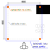
\includegraphics[width=0.6\linewidth]{kwadrat.pdf}
    \caption{Schemat ćwiczenia lotu wzdłuż prostych}
    \label{fig:kwadrat}
\end{figure}

Umiejętności wprowadzenia w zakręt, krążenia, oraz wyprowadzenia z zakrętu według doświadczeń autora są rozwijane w ramach wykonywania jednego ćwiczenia. W przeciwieństwie do manewrów opisywanych do tej pory, w tym przypadku wymagana jest pewna prędkość postępowa. Lot po okręgu wymaga wytworzenia przyspieszenia dośrodkowego o wartości proporcjonalnej do prędkości lotu. Wymagając pewnej minimalnej prędkości, utrzymanie przodu BSP w kierunku ruchu wymaga wtedy odpowiedniego przechylenie wielowirnikowca do środka zakrętu. Z tego powodu ćwiczenie rozpoczyna się od rozpędzenia w wybranym kierunku. Następnie wykonywany jest zakręt, lot wokół okręgu, wyjście z zakrętu i wyhamowanie do zawisu. Zwraca się głównie uwagę na zakreślenie równomiernego koła wokół obszaru wykonywania ćwiczeń, oraz zachowanie dynamicznego charakteru manewru. Dla stosowanego modelu wielowirnikowca arbitralnie dobrano promień koła 5~m, który po sprawdzeniu w symulacji przez autora został uznany za adekwatny. Wzajemne położenie trasy przelotu i naziemnych oznaczeń w widoku z góry ilustruje rysunek \ref{fig:kolo}.

\begin{figure}[!h]
    \centering 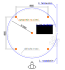
\includegraphics[width=0.8\linewidth]{kolo.pdf}
    \caption{Schemat ćwiczenia lotu w zakręcie po okręgu}
    \label{fig:kolo}
\end{figure}

\subsubsection{Implementacja w aplikacji}
Zgodnie z założeniami poczynionymi na etapie projektowania aplikacji wizualnej, dla każdego ćwiczenia przygotowano osobną scenę, w nomenklaturze silnika Unreal Engine nazywaną ,,mapą''. Aby oznaczyć miejsce zawisu umieszczono pachołek drogowy o wysokości 600~mm w odległości 7~m od operatora. Bezpośrednio nad nim znajduje się niewidoczny w trakcie ćwiczenia prostopadłościan, na rysunku \ref{fig:examhover} reprezentowany zielonymi liniami. Wlot BSP do tego obszaru rozpoczyna ocenę, zapisuje obecną wysokość jako referencyjną i rozpoczyna pomiar czasu. Niebieski znacznik orientacji umieszczony pomiędzy miejscem zawisu a operatorem wskazuje kierunek w którym należy skierować przód statku powietrznego. Po upływie 10 sekund od wejścia w zawis nad pachołkiem, ocena jest zatrzymywana, a znacznik obracany o 90°. Operator ma 10 sekund na odchylenie w nowym kierunku, po czym ocena jest wznawiana. Rozpoczęcie oceny każdorazowo jest sygnalizowane krótkim dźwiękiem. Taki cykl jest wykonywany cztery razy, dla kolejnych kursów różniących się o 90°.

\begin{figure}[!h]
    \centering \includegraphics[width=\linewidth]{examhover.png}
    \caption{Zrzut ekranu obszaru do wykonywania zawisu}
    \label{fig:examhover}
\end{figure}

Kolejne wykonywane ćwiczenie ma na celu opanowanie lotu po prostej. Identyczne pachołki drogowe jak dla oznaczenia miejsca zawisu zostały rozmieszczone w sposób opisany na rysunku \ref{fig:kwadrat}. Na wysokości 2~m nad ziemią ułożono trasę składającą się z czterech odcinków łączących kolejne wierzchołki kwadratu. Ponieważ ćwiczenie rozpoczyna się i kończy w tym samym miejscu, na każdym narożniku dodano bramki kontrolne, na rysunku \ref{fig:examsquare} widoczne jako półprzezroczyste niebieskie koła o średnicy 2~m. Poprawne ukończenie zadania wymaga przelotu przez każdą z nich. Aby czytelniej przekazać przebieg trasy, na początku ćwiczenia widoczna jest tylko bramka startu. W momencie gdy BSP znajdzie się w pobliżu przeciwległego narożnika trasy, start jest ukrywany, a zamiast tego włączana jest czerwona bramka końca.

\begin{figure}[!h]
    \centering \includegraphics[width=\linewidth]{examsquare.png}
    \caption{Zrzut ekranu obszaru do lotu po obwodzie kwadratu}
    \label{fig:examsquare}
\end{figure}

Ćwiczenie lotu w zakręcie zostało zaimplementowane w sposób bardzo zbliżony do lotu wzdłuż obwodu kwadratu. Wytyczono okrąg o średnicy i położeniu zgodnym z rysunkiem \ref{fig:kolo}. Ponieważ ćwiczenie wykonywane jest z większą prędkością, a mniejszą precyzją, podczas szkolenia praktycznego często odbywa się nieco wyżej niż pozostałe. Aby to odwzorować, trasa znajduje się na wysokości 4~m nad terenem, a bramki mają średnicę 3~m. Wygląd mapy w edytorze przedstawia rysunek \ref{fig:examcircle}. Także w tym przypadku, podczas lotu początkowo widoczna jest tylko bramka oznaczająca początek próby, a po przeleceniu połowy trasy tylko bramka końcowa.

\begin{figure}[!h]
    \centering \includegraphics[width=\linewidth]{examcircle.png}
    \caption{Zrzut ekranu obszaru do lotu w zakręcie}
    \label{fig:examcircle}
\end{figure}

\subsection{Konfiguracja systemu}
We wszystkich próbach wykorzystywany był domyślny model dynamiczny wielowirnikowca zaimplementowany w bibliotece ArduPilot SITL \cite{sitl-model}. Najważniejsze parametry modelu przedstawiono w tabeli \ref{tab:sitl-model}. Należy zwrócić uwagę, że ponieważ modelowana jest jedna konfiguracja elektrycznego statku powietrznego, masa pozostaje stała --- nie ma potrzeby rozdzielać jej na maksymalną, suchą etc.

\begin{table}[!h] \centering
    \caption{Charakterystyczne wielkości modelowanego BSP}
    \label{tab:sitl-model}

    \begin{tabular}{|l | r|l |}
    \hline
    Cecha charakterystyczna & Wielkość & Jednostka \\ \hline \hline
    Masa & 3 & kg \\ \hline
    Moment bezwładności w osi $ X $ & 0,0230 & $ \text{kg}\cdot\text{m}^2 $ \\ \hline
    Moment bezwładności w osi $ Y $ & 0,0230 & $ \text{kg}\cdot\text{m}^2 $ \\ \hline
    Moment bezwładności w osi $ Z $ & 0,0459 & $ \text{kg}\cdot\text{m}^2 $ \\ \hline
    Konfiguracja & \multicolumn{2}{c|}{\emph{quadrotor X}} \\ \hline
    Długość & 600 & mm \\ \hline
    Szerokość & 600 & mm \\ \hline
    Średnica śmigła & 350 & mm \\ \hline
    Liczba śmigieł & 4 & szt. \\ \hline
    Rozstaw śmigieł & 250 & mm \\ \hline
    Moc pobierana w zawisie & 354 & W \\ \hline
  \end{tabular}
\end{table}

Operatorzy sterowali modelem wykorzystując rzeczywisty nadajnik zdalnego sterowania \emph{FrSKY Horus X10 Express} widoczny na rysunku \ref{fig:frsky-horus}. Drążki sterowe były ustawione w układzie \emph{Mode 2}, który jest najbardziej popularny \cite{mcnabb2021}. Lewy drążek wychylany w lewo lub prawo powodował odpowiadające sterowanie w osi odchylenia. Wychylenie lewego drążka do góry zwiększa wysokość, a w dół obniża lot. Prawy drążek sterowy ma przypisane osie pochylenia i przechylenia identycznie jak w samolotach. Trzy osie, z wyjątkiem sterowania wysokością są wyposażone w sprężyny które przywracają je do położenia centralnego. Większość lotów została wykonana z wizualizacją w okularach Oculus Rift, z dwoma wyjątkami. Loty operatora Charlie oraz loty według kamery zamontowanej na BSP zostały wykonane na podstawie obrazu na płaskim monitorze komputerowym.

\begin{figure}[!h]
    \centering \includegraphics[width=0.8\linewidth]{frsky-horus.jpg}
    \caption{Wykorzystywany nadajnik zdalnego sterowania}
    \label{fig:frsky-horus}
\end{figure}

\subsection{Przebieg eksperymentu}

\subsubsection{Uczestnicy}
Uczestnicy eksperymentu wyrazili chęć ukrycia ich tożsamości w niniejszej pracy. Z tego powodu do uczestników zostały przypisane kolejne litery alfabetu. Aby uniknąć pomyłki z symbolem matematycznym zastosowanym w innej części pracy, w danych eksperymentalnych oraz opracowaniach wyników są oznaczeni wyrazami z alfabetu radiotelefonicznego ICAO. Stosowane formy męskie czasowników wynikają z gramatycznego rodzaju słowa ,,operator'', nie są powiązane z płcią uczestników. Doświadczenie poszczególnych uczestników jest przedstawione w niniejszym rozdziale, jako informacja użyteczna w analizie uzyskanych wyników.

Podsumowując, w grupie znalazło się trzech uczestników bez żadnego doświadczenia w pilotażu BSP oraz czterech którzy wcześniej wykonywali loty. Spośród uczestników z doświadczeniem, wszyscy wykonywali wcześniej loty wielowirnikowcami. Dwóch z nich posiada świadectwo kwalifikacji.

Operator Alfa nie miał wcześniej doświadczenia związanego z pilotażem BSP. Jako jedyny zgłosił, że regularnie gra w gry komputerowe.

Operator Bravo przed badaniem kilkukrotnie wykonywał loty BSP typu wielowirnikowiec wyposażonym w układ autopilota, każdorazowo wykorzystując automatyczną stabilizację pozycji opartą o system GNSS. Ostatnie loty wykonywał ponad 12 miesięcy przed badaniem.

Operator Charlie nie miał wcześniej doświadczenia związanego z pilotażem BSP. Jako jedyny nie wykonywał lotów w okularach VR.

Operator Delta nie miał wcześniej doświadczenia związanego z pilotażem BSP.

Operator Echo przed badaniem wykonywał loty BSP typu wielowirnikowiec wyposażonym w układ autopilota, każdorazowo wykorzystując automatyczną stabilizację pozycji opartą o system GNSS. Uzyskał uprawnienia BVLOS w kategorii szczególnej. Ostatnie loty wykonywał ponad 4 miesiące przed badaniem.

Operator Foxtrot przed badaniem kilkukrotnie wykonywał loty BSP typu wielowirnikowiec wyposażonym w układ autopilota, każdorazowo wykorzystując automatyczną stabilizację pozycji opartą o system GNSS. Ostatnie loty wykonywał w miesiącu badania.

Operator Golf (autor pracy) przed badaniem wykonywał loty BSP różnych typów, z układami autopilota oraz bez żadnej automatycznej stabilizacji. Ostatnie loty wykonywał ponad 2 miesiące przed badaniem. Jako jedyny korzystał z utworzonego systemu przed przeprowadzeniem badania. Wpływ doświadczenia zdobytego w systemie został zminimalizowany, przez sprawdzanie funkcjonalności bez podłączania symulacji AP~SITL. Poza badaniem wykorzystywano trywialny model kinematyczny, w którym naciśnięcie przycisku na klawiaturze komputera powodowało przemieszczanie symulowanego BSP ze stałą prędkością.

\subsubsection{Wykonane loty}
Pierwotnie przygotowany plan zadań do wykonania w trakcie badania musiał zostać zmodyfikowany, aby dostosować go do umiejętności uczestników. Według doświadczenia autora, podczas tradycyjnego szkolenia nauka zawisu bez automatycznej stabilizacji pozycji zajmuje około kilkudziesięciu minut. Niestety, czas który uczestnicy mogli poświęcić na badania był bardzo ograniczony. Różniąca się liczba lotów wynika głównie z tego czynnika. W tabeli \ref{tab:loty} zebrano wszystkie loty zapisane w trakcie badania, z których będą wybierane odpowiednie podzbiory w opracowaniu wyników.

\begin{table}[!h] \centering
    \caption{Podsumowanie wszystkich lotów zebranych w trakcie badań}
    \label{tab:loty}
    \renewcommand{\arraystretch}{1.3} % Wyższe o 30% rzędy tabeli

    \begin{tabular}{| l *{7}{| c} |}
        \hline
        \textbf{Rodzaj lotu} &
        \spheading[5em]{Alfa} &
        \spheading[5em]{Bravo} &
        \spheading[5em]{Charlie} &
        \spheading[5em]{Delta} &
        \spheading[5em]{Echo} &
        \spheading[5em]{Foxtrot} &
        \spheading[5em]{Golf} \\ \hline \hline
        Zawis z GNSS               & 1 & 1 & 1 & 2 & 1 &   & 1 \\ \hline
        Zawis bez GNSS, bez wiatru & 2 & 1 & 1 & 1 & 1 &   & 2 \\ \hline
        Zawis bez GNSS, z wiatrem  & 6 & 6 & 2 &   & 5 &   & 6 \\ \hline
        j. w., przerwana próba     &   &   & 2 & 4 & 1 & 2 &   \\ \hline
        Kwadrat z GNSS             & 6 & 6 &   & 1 & 1 &   &   \\ \hline
        Koło z GNSS                & 4 &   &   &   &   &   & 3 \\ \hline
        Koło z GNSS, widok FPV     & 2 &   &   &   &   &   & 2 \\ \hline
    \end{tabular}
\end{table}

Opisane w tabeli rodzaje lotów były wykonywane z różnymi ustawieniami autopilota. W lotach oznaczonych ,,z GNSS'' był aktywny tryb \emph{LOITER}, w którym autopilot utrzymuje ostatnio zadaną pozycję poziomą. Wychylenie prawego drążka sterowego należy interpretować jako \emph{position command}, czyli przemieszczanie punktu w którym sterownik ma utrzymywać statek powietrzny. Wszyscy operatorzy deklarowali, że wpływ wiatru w tym trybie jest niezauważalny. Podczas lotów opisanych ,,bez GNSS'' autopilot pracował w trybie \emph{ALT\_HOLD}, w którym nie jest zachowywane stałe położenie. Wychylenie prawego drążka jest odczytywane jako \emph{attitude command}, czyli powoduje pochylenie i przechylenie BSP. W przeciwieństwie do trybu \emph{LOITER}, po puszczeniu sterownic BSP wróci do położenia poziomego, ale będzie się przemieszczał z dotychczasową prędkością z przyspieszeniem wynikającym z wiatru i siły oporów aerodynamicznych. Wysokość oraz kąt odchylenia w obu trybach były utrzymywane automatycznie, operator miał możliwość sterować w obu tych osiach za pomocą lewego drążka sterowego.

We wszystkich ćwiczeniach w których występował wiatr, wiał z prędkością $ 2 \frac{\text{m}}{\text{s}} $ stałą niezależnie od położenia i czasu. Wyłączono turbulencje oraz efekt przyziemny, powodujący zwiększanie się prędkości wiatru wraz ze zwiększaniem wysokości nad podłożem. W trakcie jednego lotu kierunek pozostawał stały, ale był zmieniany pomiędzy kolejnymi podejściami do tego samego ćwiczenia. Ponieważ zawis jest wykonywany w czterech orientacjach, a operatorzy określali kompensację ukośnego kierunku wiatru jako trudniejszą, zastosowano algorytm tworzący serię niewymiernych, niepowtarzających się kątów. W pierwszej kolejności kąt pełny jest dzielony na dwie części według zasady złotego podziału, a do następnych obliczeń zapisywany jest mniejszy z tak otrzymanych kątów. Tę wartość opisano w równaniu \ref{eq:zlotypodzial} literą $ \alpha $. Przemieszczając się wzdłuż obwodu koła o ten kąt, uzyska się najbardziej niewymierny rozkład punktów na okręgu \cite{ridley1982}. Na pierwszy kierunek wiatru przyjęto 180°, czyli zza pleców operatora. Spośród czterech kierunków kardynalnych ten wybrano na najłatwiejszy, ponieważ dryfujący BSP pozostaje w polu widzenia. Zbiór kierunków wiatru które wykorzystano przy wykonanej ilości prób przedstawiono na rysunku \ref{fig:wiatr}.

\begin{align}
    \label{eq:zlotypodzial}
    \begin{cases}
        \frac{\alpha}{\beta} = \frac{\beta}{360^{\circ}} \\
        \alpha + \beta = 360^{\circ}
    \end{cases} \Rightarrow \frac{\beta}{\alpha} = \phi &\approx 1.61803\dots
    \\
    \alpha &\approx 137.508^{\circ}
\end{align}

\begin{figure}[!h]
    \centering 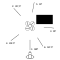
\includegraphics[width=0.6\linewidth]{wiatr.pdf}
    \caption{Kierunki wiatru wykorzystywane w próbach zawisu}
    \label{fig:wiatr}
\end{figure}

Próby były przerywane w przypadku gdy uczestnik po oddaleniu się BSP na znaczną odległość, deklarował że nie jest w stanie powrócić do miejsca wykonywania ćwiczenia. Ćwiczenie lotu po okręgu wymagało najbardziej złożonej nawigacji w porównaniu do pozostałych dwóch. Podczas podejść w widoku FPV obserwowano wizualizację z kamery przemieszczającej się razem z BSP, tworząc wrażenie podobne do siedzenia w kokpicie załogowego statku powietrznego.

Wynikiem każdej z prób jest plik tekstowy w formacie CSV zawierający wszystkie zebrane dane. Nadajnik operatora wykorzystywany w próbie jest bezpośrednio połączony z symulacją BSP. Następnie stan symulacji jest przesyłany protokołem MAVLink do wizualizacji i wyświetlany na okularach operatora. Położenie, orientacja przestrzenna, prędkość statku powietrznego oraz odległość od trasy referencyjnej są zapisywane dla każdej wyświetlonej klatki obrazu oraz wysyłane do oceny. Serwer oceny oblicza poszczególne składowe błędu, oraz odsyła wiadomość z wynikami do aplikacji wizualnej. Wyniki oceny są przypisywane do odpowiedniego stanu na podstawie znacznika czasu, dzięki czemu mogą być zapisane w tym samym wierszu pliku z wynikami. Dalsza obróbka danych może być zrealizowana w dowolnym pakiecie obliczeniowym. Z powodu znacznej liczby plików, w niniejszej pracy wykorzystano \cite{soft:pandas} do analizy wyników i przygotowania wykresów.

\subsection{Wyniki}
Zadanie zawisu na wietrze, bez stabilizacji pozycji zostało wykonane przez wszystkich uczestników badania. Poziom trudności tego zadania spowodował największą różnicę w wynikach. Zebrane oceny przedstawiono w tabeli \ref{tab:oceny}. Należy zwrócić uwagę, że zgodnie z definicjami w tabeli \ref{tab:ocena-funkcje} lepszy lot oznacza niższą wartość oceny. Te same dane rozdzielone na ocenę pozycji oraz kąta odchylenia przedstawia wykres na rysunku \ref{fig:plot-ocena}. Zgodnie z definicją funkcji oceny, każdy operator wykonywał to zadanie przez ten sam okres czasu. Próby które zostały przerwane przez utratę kontroli nie spełniały tego warunku, dlatego nie została dla nich obliczona ocena.

\begin{table}[!h] \centering
    \caption{Oceny przypisane operatorom w zawisie na wietrze}
    \label{tab:oceny}
    \renewcommand{\arraystretch}{1.3} % Wyższe o 30% rzędy tabeli

    \begin{tabular}{| r *{8}{| c } |}
        \hline
        \textbf{Kolejne podejście} &
        \spheading[5em]{Alfa} &
        \spheading[5em]{Bravo} &
        \spheading[5em]{Charlie} &
        \spheading[5em]{Delta} &
        \spheading[5em]{Echo} &
        \spheading[5em]{Foxtrot} &
        \spheading[5em]{Golf} \\ \hline \hline
        1                &  44.41 & 23.41 &   P   & P &   P   & P & 1.87 \\ \hline
        2                & 100.92 & 25.48 & 77.72 & P & 25.08 & P & 2.52 \\ \hline
        3                &  23.43 & 26.90 & 67.72 & P & 34.78 &   & 1.26 \\ \hline
        4                &  12.41 & 15.20 &   P   & P & 48.60 &   & 3.91 \\ \hline
        5                &  53.31 & 35.76 &       &   & 12.89 &   & 2.26 \\ \hline
        6                &  44.46 & 25.07 &       &   & 74.11 &   & 3.91 \\ \hline\hline
        \textbf{średnia} &  46.49 & 25.30 & 72.72 &   & 39.09 &   & 2.62 \\ \hline
    \end{tabular}
\end{table}

\begin{figure}[!h]
    \centering \includegraphics[width=\linewidth]{plot-ocena.pdf}
    \caption{Wykres ocen operatorów rozdzielony na składowe}
    \label{fig:plot-ocena}
\end{figure}

Na podstawie dokonanej oceny można wysunąć kilka wniosków. Nie sprawdziła się hipoteza stawiana w podrozdziale \ref{sec:wybrane-cwiczenia}, że wyniki uczestników będą coraz lepsze wraz z kolejnymi podejściami. Prawdopodobnie wynika to z niewielkiej ilości doświadczenia które zdobyli w trakcie badań. Próby były wykonywane bezpośrednio po sobie, po wczytaniu zadania z nowym kierunkiem wiatru uczestnicy mieli się zaznajomić z warunkami i rozpocząć oceniany manewr kiedy będą gotowi.

Można zaobserwować zbieżność przyznanej oceny z poziomem doświadczenia uczestników badania. Na potrzeby tego porównania, każdej przerwanej próbie zostanie przypisany najgorszy wynik osiągnięty w ukończonym ćwiczeniu, czyli $ 100.92 $. Po takim poszerzeniu dostępnych danych, grupa operatorów Alfa, Charlie i Delta którzy po raz pierwszy pilotowali BSP osiągali średni wynik $ 73.56 $. Operatorzy Bravo, Echo i Foxtrot którzy mieli doświadczenie z BSP, ale brak ćwiczenia w sterowaniu ręcznym, średnio uzyskali znacząco lepszy wynik $ 43.46 $. Niestety tylko operator Golf miał wcześniejsze doświadczenia w ręcznym pilotowaniu. Skrajnie mała próbka uniemożliwia jednoznaczną identyfikację czynników które spowodowały że średnia ocena wyniosła tylko $ 2.622 $.

Jak można zaobserwować na wykresie \ref{fig:plot-ocena} znacznie większe różnice pomiędzy operatorami były widoczne w zakresie sterowania położeniem BSP. Poza kilkoma gorszymi podejściami, sterowanie w kanale odchylenia było wykonywane bardzo poprawnie. Kolejne orientacje w których należało wykonywać zawis różniły się od siebie o 90°. Na histogramie przedstawionym na rysunku \ref{fig:plot-yaw-histogram} widać że oprócz malejącej częstotliwości dla większych wartości błędu, widać lokalne maksimum w okolicach właśnie 90°. Najprawdopodobniej odpowiada to sytuacjom w których operator nie wykonał obrotu w trakcie przeznaczonego na to czasu.

\begin{figure}[!h]
    \centering \includegraphics[width=0.8\linewidth]{plot-yaw-histogram.pdf}
    \caption{Histogram wartości błędu w osi odchylenia}
    \label{fig:plot-yaw-histogram}
\end{figure}

Aby lepiej przedstawić rozkład błędu w następujących rozważaniach zostanie wykorzystany wykres pudełkowy\footnote{ang. \emph{box-plot}}. Dla każdego zestawu próbek jest rysowany prostokąt, którego dolna i górna granica oznaczają odpowiednio pierwszy i trzeci kwartyl wartości. Pozioma linia wewnątrz prostokąta jest umieszczona na wysokości mediany. Odcinki na zewnątrz prostokąta zwane ,,wąsami'', w tej pracy zawsze oznaczają 2 oraz 98 centyl. Z powodu dużej ilości próbek podlegających ocenie, elementy odstające nie są rysowane ponieważ znacznie pogarszały czytelność.

Na rysunku \ref{fig:plot-operator-pos-box} przedstawiono wartości błędu położenia BSP w kolejnych klatkach symulacji, tj. próbkowane z częstotliwością 45~Hz. Zostały wybrane ze wszystkich ukończonych prób zawisu przy wietrze, oraz pogrupowane według operatorów. Można zaobserwować że mediana dla wszystkich serii oprócz Golf znajduje się na bardzo podobnym poziomie: $ 2.88 \pm 0.13 \text{m} $, ale różnią się górną granicą. Fakt że przypisano im znacznie różniące się oceny, wskazuje na osiągnięcie celu penalizowania dużych błędów wskazanego w rozdziale \ref{sec:dobor-kryteriow}.

\begin{figure}[!h]
    \centering \includegraphics[width=0.8\linewidth]{plot-operator-pos-box.pdf}
    \caption{Charakterystyka błędu pozycji według operatorów}
    \label{fig:plot-operator-pos-box}
\end{figure}

Oprócz porównania między sobą poszczególnych operatorów, zbadano wpływ różnych warunków na trudność wykonywania manewru zawisu. Jak widać na wykresie \ref{fig:plot-wind-pos-box}, kierunek wiatru nie miał dużego wpływu na wyniki, chociaż potwierdziła się teza, że wiatr wprost za pleców będzie najłatwiejszy do skompensowania.

\begin{figure}[!h]
    \centering \includegraphics[width=0.8\linewidth]{plot-wind-pos-box.pdf}
    \caption{Charakterystyka błędu pozycji względem wiatru}
    \label{fig:plot-wind-pos-box}
\end{figure}

Podczas badań operatorzy wielokrotnie komentowali, że zawis w orientacjach innych niż przodem BSP w kierunku patrzenia jest znacznie trudniejszy, w szczególności przodem do operatora. Stany lotu pogrupowano według najbliższej wielokrotności 90° w osi odchylenia, a wyniki przedstawiono na rysunku \ref{fig:plot-orientation-pos-box}. Wartości błędu potwierdzają że zawis przodem BSP ,,od siebie'' faktycznie jest najłatwiejszy, ale w przeciwieństwie do subiektywnych opinii nie widać znaczącej różnicy w pozycji odwróconej.

\begin{figure}[!h]
    \centering \includegraphics[width=0.8\linewidth]{plot-orientation-pos-box.pdf}
    \caption{Charakterystyka błędu pozycji względem orientacji BSP}
    \label{fig:plot-orientation-pos-box}
\end{figure}

Zdecydowanie czynnikiem najsilniej wpływającym na trudność utrzymania pozycji jest konieczność prowadzenia stałych poprawek. W przypadku stabilizacji pozycji na podstawie wskazań symulowanego GNSS, operatorzy musieli jedynie dolecieć w odpowiednim miejsce, a następnie obracać w osi odchylenia zgodnie z poleceniami. Zawis bez GNSS w bezwietrznym powietrzu wymaga samodzielnego zatrzymania BSP w odpowiednim punkcie, sterując w zasadzie przyspieszeniem w kierunku poziomym. Po wytraceniu całej prędkości nad znacznikiem, wystarcza obracanie i okazjonalne korekty.

Ręczne sterowanie pochyleniem i przechyleniem przy wietrze jest znacznie większym obciążeniem dla operatora. Konieczne są ciągłe poprawki w celu utrzymania BSP w jednym miejscu. Zachowanie stałej prędkości wymaga znalezienia takiego wychylenia drążka sterowego żeby pozioma składowa siły ciągu równoważyła napór wiatru. Ponadto po każdej zmianie orientacji BSP, równowaga jest osiągnięta przy innym położeniu sterownicy. Na wykresie \ref{fig:plot-task-pos-box} wyraźnie widać pogarszające się wyniki wraz z rosnącą ilością poprawek wymaganych od operatora.

\begin{figure}[!h]
    \centering \includegraphics[width=0.8\linewidth]{plot-task-pos-box.pdf}
    \caption{Charakterystyka błędu pozycji względem stabilizacji wymaganej od operatora}
    \label{fig:plot-task-pos-box}
\end{figure}

Ostatnim czynnikiem którego wpływ sprawdzono, jest perspektywa z której operator obserwuje położenie BSP względem zadanej ścieżki. Dane przedstawione na wykresie \ref{fig:plot-fpv-pos-box} jako jedyne w tym podrozdziale zostały zebrane w trakcie lotu po okręgu. Można zaobserwować że prowadzenie statku powietrznego jest łatwiejsze na podstawie widoku z wnętrza, ale nie jest to tak duża różnica jak przewidywano.

\begin{figure}[!h]
    \centering \includegraphics[width=0.8\linewidth]{plot-fpv-pos-box.pdf}
    \caption{Charakterystyka błędu pozycji względem perspektywy obserwacji}
    \label{fig:plot-fpv-pos-box}
\end{figure}

\newpage
\section{Plan dalszego rozwoju}
\begin{todo}
    Wskazać możliwość dodawania zadań, innych funkcji oceny itp. Opisać sposób przejścia na AR. Podłączanie różnych symulacji - praca Ł. Grabowskiego. Opisać prace zespołu w projekcie Boeing.
\end{todo}
\newpage
\section{Podsumowanie}

\subsection{Ocena wyników}
\begin{todo}
    Odwołanie się do wymagań wobec projektu i wskazanie sposobów realizacji.
\end{todo}

\subsection{Wykorzystane narzędzia}
\begin{todo}
    Oprogramowanie open-source, licencje na poszczególne składniki
\end{todo}

\subsection{Podziękowania}

%--------------------------------------------
% Literatura
%--------------------------------------------
\cleardoublepage % Zaczynamy od nieparzystej strony
\printbibliography

%--------------------------------------------
% Spisy (opcjonalne)
%--------------------------------------------
\newpage
\pagestyle{plain}

% Wykaz symboli i skrótów.
% Pamiętaj, żeby posortować symbole alfabetycznie
% we własnym zakresie. Ponieważ mało kto używa takiego wykazu,
% uznałem, że robienie automatycznie sortowanej listy
% na poziomie LaTeXa to za duży overkill.
% Makro \acronymlist generuje właściwy tytuł sekcji,
% w zależności od języka.
% Makro \acronym dodaje skrót/symbol do listy,
% zapewniając podstawowe formatowanie.
% //AB
\vspace{0.8cm}
\acronymlist
\acronym{AR}{Augmented Reality}
\acronym{BSP}{Bezzałogowy Statek Powietrzny}
\acronym{CSV}{Comma-Separated Values}
\acronym{FPV}{First Person View}
\acronym{IP}{Internet Protocol}
\acronym{JSON}{JavaScript Object Notation}
\acronym{TCP}{Transmission Control Protocol}
\acronym{VR}{Virtual Reality}

\listoffigurestoc     % Spis rysunków.
\vspace{1cm}          % vertical space
\listoftablestoc      % Spis tabel.
\vspace{1cm}          % vertical space
\listofappendicestoc  % Spis załączników

% Tabele i wykresy w załączniku nie są brane pod uwagę w spisie tabel i wykresów.
% Ich numeracja jest zresetowana.
\captionsetup[figure]{list=no}
\captionsetup[table]{list=no}

% Załączniki
% \newpage
% \appendix{Nazwa załącznika 1}
% \lipsum[1-4]

% Używając powyższych spisów jako szablonu,
% możesz tu dodać swój własny wykaz bądź listę,
% np. spis algorytmów.

\end{document} % Dobranoc.
